% !TEX program = xelatex
% !TEX encoding = UTF-8 Unicode
% !BIB program = biber
\documentclass[english]{textolivre}



% metadata
\journalname{Texto Livre}
\thevolume{17}
%\thenumber{1} % old template
\theyear{2024}
\receiveddate{\DTMdisplaydate{2024}{5}{21}{-1}}
\accepteddate{\DTMdisplaydate{2024}{6}{22}{-1}}
\publisheddate{\DTMdisplaydate{2024}{11}{6}{-1}}
\corrauthor{Hussein Abu-Rayyash}
\articledoi{10.1590/1983-3652.2024.52687}
%\articleid{NNNN} % if the article ID is not the last 5 numbers of its DOI, provide it using \articleid{} commmand 
% list of available sesscions in the journal: articles, dossier, reports, essays, reviews, interviews, editorial
\articlesessionname{articles}
\runningauthor{Abu-Rayyash; Alhawamdeh and Ringomon}
%\editorname{Leonardo Araújo} % old template
\sectioneditorname{Daniervelin Pereira}
\layouteditorname{João Mesquita}

\title{The eye-ear relationship: investigating auditory impacts on subtitle reading and comprehension}
\othertitle{A relação olho-ouvido: investigando os impactos auditivos na leitura e compreensão de legendas}

\author[1]{Hussein Abu-Rayyash ~\orcid{0000-0002-9695-4030  }\thanks{Email: \href{mailto:haburayy@kent.edu }{haburayy@kent.edu }}}
\author[1,2]{Shatha Alhawamdeh~\orcid{0009-0001-6342-7242}\thanks{Email: \href{mailto:salhawam@kent.edu}{salhawam@kent.edu}}}
\author[1]{Yuri Ringomon~\orcid{0009-0000-6508-8769}\thanks{Email: \href{mailto:yringomo@kent.edu }{yringomo@kent.edu }}}
\affil[1]{Kent State University, College of Arts and Sciences, Department of Modern and ClassicalLanguage Studies, Kent, Ohio, USA.}
\affil[2]{Oberlin College, College of Arts and Sciences, Department of Middle East and North Africa Studies, Oberlin, Ohio, USA.}

\addbibresource{article.bib}
\usepackage{tabularx,multirow}%,makecell}%,multirow}

\newcolumntype{Y}{>{\centering\arraybackslash}X}
%\usepackage{longtable}

\setotherlanguage{arabic}
\newfontfamily\arabicfont[Script=Arabic]{Amiri}
\newfontfamily\arabicfontsf[Script=Arabic]{Amiri}
\newfontfamily\arabicfonttt[Script=Arabic]{Amiri}

\begin{document}
\maketitle
\begin{polyabstract}
\begin{abstract}
  The study employs eye-tracking measures and comprehension
  quizzes to investigate linguistic processing during subtitle reading and
  comprehension in Arabic and Spanish. Specifically, it examines the
  impact of native English (L1) audio, foreign Spanish or Arabic (L2)
  audio, or the absence of audio on subtitle reading strategies and the
  processing of embedded linguistic units in novice learners. The study
  utilizes a 2x3 within-subjects design, manipulating audio condition (L1
  audio, L2 audio, no audio) and subtitle language (Spanish, Arabic).
  Global eye-tracking analyses reveal subtitle reading patterns, while
  local analyses focus on the processing of specific linguistic units.
  Comprehension quizzes assess learning outcomes after the viewing of the
  subtitled videos. The findings suggest that the absence of audio leads
  to increased fixation durations, indicating greater attentional demand.
  Spanish subtitles result in higher fixation counts and prolonged reading
  times compared to Arabic, reflecting deeper cognitive processing. The
  study highlights the complex interplay between audio presence, subtitle
  language, and individual proficiency in shaping attentional allocation
  and lexical processing during language acquisition through audio-visual
  media.
\keywords{Eye Movement \sep Audio \sep Subtitles \sep Reading \sep Comprehension}
\end{abstract}

\begin{portuguese}
\begin{abstract}
O estudo emprega medidas de rastreamento ocular e
questionários de compreensão para investigar o processamento linguístico
durante a leitura e compreensão de legendas em árabe e espanhol.
Especificamente, examina o impacto do áudio nativo em inglês (L1), áudio
estrangeiro em espanhol ou árabe (L2) ou a ausência de áudio nas
estratégias de leitura de legendas e no processamento de unidades
linguísticas inseridas em aprendizes iniciantes. O estudo utiliza um
delineamento intra-sujeitos 2x3, manipulando a condição de áudio (áudio
L1, áudio L2, sem áudio) e a língua das legendas (espanhol, árabe). As
análises globais de rastreamento ocular revelam padrões de leitura de
legendas, enquanto as análises locais se concentram no processamento de
unidades linguísticas específicas. Os questionários de compreensão
avaliam os resultados de aprendizagem após assistir aos vídeos
legendados. Os resultados sugerem que a ausência de áudio leva a um
aumento na duração das fixações, indicando uma maior demanda atencional.
As legendas em espanhol resultam em um maior número de fixações e tempos
de leitura prolongados em comparação com o árabe, refletindo um
processamento cognitivo mais profundo. O estudo destaca a complexa
interação entre a presença de áudio, a língua das legendas e a
proficiência individual na alocação de atenção e no processamento
lexical durante a aquisição de línguas através de mídia audiovisual.

\keywords{Movimento Ocular \sep Áudio \sep Legendas \sep Leitura \sep Compreensão}
\end{abstract}
\end{portuguese}

\end{polyabstract}

\section{Introdução}\label{sec-introdução}
O canal Porta dos Fundos tem um vídeo chamado Excêntrico, de 2015. Ele se inicia com um homem sentado em seu sofá quando seus amigos entram assustados em seu apartamento, trazendo bombeiros e outros homens, em sobressalto fazendo parecer que precisaram arrombar a porta. Eles estavam preocupados porque esse homem não havia respondido a um \textit{e-mail} que havia sido enviado há mais de duas horas, nem respondido a mensagens em diversas redes sociais nesse meio tempo. Os amigos dizem que achavam que ele poderia ter sido sequestrado porque, afinal, quem é que fica \enquote{tanto tempo} offline atualmente? O homem estava em casa, lendo um livro, motivo pelo qual é chamado de \textit{vintage} por um dos colegas. 

\enquote{Excêntrico}, o título do vídeo, refere-se, segundo o Dicionário Aurélio da Língua Portuguesa, ao indivíduo original, extravagante ou esquisito. Depreende-se daí que, na sociedade em que vivemos, desconectar-se é ser excêntrico e, por oposição, que o padrão estabelecido seja o da conexão ininterrupta. Este é o cenário que nos cerca hoje, no século XXI. Cabe ainda observar que o vídeo foi feito em 2015, quase uma década atrás, e desde então essa conexão tem se intensificado e se estendido para mais âmbitos da vida, em especial depois de 2020, como efeito da pandemia de Covid-19.

\section{Literature Review}\label{sec-literaturereview}

Enhancing students' reading comprehension skills has emerged as a
significant concern in both academic and non-academic settings \cite{kim2023}. Translation plays a crucial role in enhancing reading
comprehension, as noted by \textcite{alaboud2022}, who found that "translation
could be an effective instructional strategy in improving
learners\textquotesingle{} skills in reading comprehension in an EFL
setting" \textcite[p. 424]{alaboud2022}. In a case study of medical students,
\textcite{rushwan2017} indicated that the use of translation can facilitate and
enhance reading comprehension skills of ESP medical learning. Concerning
the utilization of subtitles to improve reading skills, several studies
\cite{omar2023,qazi2023} have endorsed the notion that
audio-visual materials enriched with subtitles manifest to enhance both
second language (L2) reading comprehension abilities. For instance,
\textcite{haider2022} indicate that the effects of viewing
captioned videos on EFL learners revealed a positive impact on reading
comprehension. \textcite{xu2022} also state that utilizing videos serves
as a potent and engaging educational resource for EFL learners. In their
study, Xu et al. provide further insights into the impact of viewing
captioned videos on the listening and reading skills of university EFL
learners. While the reading of subtitles has garnered increasing
attention in recent decades, our comprehension of the cognitive
processes involved in subtitle reading, and the variances from reading
static text, remains constrained \cite{baranowska2020}. Research in
subtitle reading has been significantly influenced by the intersection
of auditory input and visual processing. The relationship between what
viewers hear and what they read on screen presents intriguing questions
about cognitive workload and language comprehension.

To take in new information, our eyes must adjust their focal direction
to where it is most concerned next, ``in order to process information
most effectively we must move our eyes so that the fovea fixates the
location of that which we intend to process'' \cite[p. 84]{schotter2012}. One cannot presume that eye engagement behavior remains
static throughout the language learning endeavor \cite{blythe2005}.
\textcite[p. 86]{schotter2012} emphasize that ``Interestingly, the
amount of disparity {[}between individual eye focus{]} tends to be
greater in beginning readers than skilled readers''. Thus, our research
seeks to tackle this trend early in the language learning process for
second language learners. The pace at which they can become more fluent
may differ and be faster than the pace they had when they learned their
first language; however, such learners would be susceptible to
individual eye focus disparity. Subtitles presentation through the
purposeful utilization of colors, size, spacing, font and timing could
have a varying degree of impact when considering these factors. In
addition, video and subtitle speed is also an impactful factor upon the
viewer. According to \textcite{liao2020}, as subtitle speed increases,
word frequency and word length effects become less pronounced in local
eye movement measures marking lexical processing. The authors conclude
that increasing subtitle speed results in a shift "from local
(cognitive) eye-movement control towards heuristics informed by global
task constraints (e.g., subtitle speed)" \textcite[p. 430]{liao2020}.
This suggests that attention allocation during subtitle reading relies
less on characteristics of individual words when subtitles are presented
more rapidly.

Studies by \textcite{ross2023} and \textcite{szarkowska2018}
highlight a trend where the presence of audio, especially in a viewer's
native language, leads to reduced reliance on subtitles. This phenomenon
suggests that audio can support and enhance the subtitle reading
experience, particularly when it is semantically aligned with the text.
Another key consideration to be aware of is that the overall ``reading
process could be affected by semantically relevant auditory input in the
context of reading English/L2 subtitles in video'' \cite[p. 259]{liao2020}.

\textcite{liao2022} present evidence that in situations involving
multimodal reading, like reading subtitles in videos, eye movements are
not solely regulated by visual information. Rather, readers
simultaneously incorporate inputs from both visual and auditory
modalities in the moment to determine when, where, and even whether to
shift their eyes for subtitle reading. Thus, \textcite{liao2022}
contribute to this discourse by examining how auditory input, even when
partially redundant, influences the comprehension of subtitled content.
Their study moves beyond the mere tracking of eye movements to consider
how the audio-visual synergy affects viewers\textquotesingle{}
higher-level understanding of content.

A gap still exists in understanding the specific dynamics of how
auditory context facilitates subtitle reading. \textcite{ragni2020} partially
addressed this by investigating second-language subtitles with native
language audio. Yet, the absence of a no-audio condition in
Ragni\textquotesingle s research limits the ability to discern the
exclusive effects of auditory input on subtitle processing.

Given the widespread use of subtitles in second language education,
understanding how audio influences subtitle comprehension is critically
important. A range of prior research, as summarized by \textcite{liao2022}, has studied the impacts of native and foreign language audio on
global subtitle reading approaches using eye-tracking measures with
languages like Dutch, Swedish, and English. Other work also revealed the
effects of varied audio backing on patterns indicative of reading
strategies \cite{szarkowska2018}. Additionally, recent
studies measured local lexical and perceptual processing through
fixation metrics \cite{bisson2014,ragni2020}.

\textcite{bravo2008} extensively examined audiovisual-based language
learning. In her work, Bravo emphasizes that subtitles should not be
viewed as a panacea for foreign language acquisition. Despite the
wealth of research on how audiovisual configurations affect second
language learning, this topic remains relevant to related disciplines,
particularly linguistics and translation studies, which in turn
influence second language acquisition. Historically, translation has
been employed in second language instruction by formal educational
institutions. Furthermore, individual language learners have used
translation as a method to test and improve their comprehension of the
target language.

The current study builds upon these precedents by isolating the impacts
of native English audio, foreign Spanish/Arabic audio, and no audio
conditions during Spanish and Arabic subtitle reading specifically for
novice learners. The investigation goes beyond prior global analyses to
align macro reading strategies with granular dynamic time courses of
vocabulary integration efficiency. Through coordinated examination of
sentence-level and localized word-level processing, the work
comprehensively evaluates the contributions of audio presence and
language proximity factors to literacy development gains.

While \textcite{borrás1994} found that the opportunity of having
subtitles has a positive impact on comprehension, they also claim that
it improves the productive use of the foreign language. A factor that is
not underscored within this particular study, though it is of great
consequence upon second language acquisition, is individual writing
skill. In writing, phrasal usage is promoted as being a strategy that
enhances the quality of a text. This is not only true for English, but
also stressed in the Arabic writing system \cite{anis2022}. The
videos used in this experiment certainly had phrases, and the
participants may or may not have caught on to the phrases. \textcite{anis2022} found that the translations of Arabic literature (primarily
poetry, in their example) can be done more naturally if the Arabic
source text has phrases. Perhaps this finding then would also support a
notion that suggests that phrasal usage in oral speech in videos could
potentially be noticed by the listeners even if the language is their L2
language.

This eye-tracking study explores the impacts of native English language
(L1) versus foreign Spanish or Arabic language (L2) auditory input, or
its absence, on Spanish or Arabic subtitle reading and comprehension.
The research utilizes a 2x3 within-subjects design with native
English-speaking learners, manipulating audio condition (L1 English
audio present, L2 Spanish or Arabic audio present, or no audio) and
evaluating the effects on Spanish or Arabic subtitle processing.

The study aims to answer three questions:

1. How do L1 English audio, L2 Spanish or Arabic audio, and no audio
conditions influence global subtitle reading efficiency patterns and
local lexical processing in novice learners?

2. What is the relationship between L1 English or L2 Spanish or Arabic
auditory input and comprehension accuracy with Spanish or Arabic
subtitled foreign language content?

3. Does the presence or absence of L1 English versus L2 Spanish or
Arabic audio impact perceived cognitive load during Spanish or Arabic
subtitle reading?
\section{Methodology}\label{sec-methodology}

This section presents an overview of the methodology used in the study.
It includes details about the sample and data collection and analysis
processes. The study employs quantitative measures to investigate
subtitle reading and comprehension in novice learners of Spanish and
Arabic. Quantitative data is gathered through eye-tracking measures and
comprehension quizzes to analyze participants\textquotesingle{} reading
patterns and learning outcomes. Our methodological approach differs,
though not to a radical degree, from that of Martínez and Gomez (2020),
who found that competency in oral understanding of L2 intake increased
through the usage of audio-visual tools and streaming services that use
them. The following subsections of section 3 will provide more detail on
the methodology.

\subsection{Participants}\label{sub-sec-participants}

The study involves 30 participants, comprising 20 native
English-speaking university students as beginner learners of Spanish and
10 beginner learners of Arabic. All participants have studied their
respective language (Spanish or Arabic) for only 1-2 semesters at the
university level. To ensure a broad and unbiased participant pool, the
recruitment phase involves outreach to language instructors.
Participants are aged between 18-40 years to control for age-related
cognitive and oculomotor changes. In accordance with Institutional
Review Board guidelines, informed consent is obtained, along with
assurances of data confidentiality and ethical handling of participant
information. A pilot test with 5 participants is conducted to refine the
study methodology, ensuring clarity in instructions and overall
procedure.

\subsection{Design}\label{sub-sec-design}

The study employs a 2x3 within-subjects design to assess the impact of
subtitle language combined with auditory input. The study manipulated
audio condition (L1 audio, L2 audio, no audio) and subtitle language
(Spanish, Arabic). This design features 2 levels of subtitle language
(Spanish and Arabic) crossed with 3 types of audio exposure (L1 English
Audio, L2 Matched Audio, No Audio). Each native English participant,
either a Spanish learner or an Arabic learner, completes 3 total viewing
conditions specific to their language of study (L2: Spanish/Arabic) (see
\Cref{tab-01}). To ensure the reliability of the results and counter potential
biases, the sequence in which participants encounter these conditions is
randomized, controlling for order effects and fatigue. This strategy is
crucial for reducing learning or adaptation effects across sessions.

Eye-tracking data were collected using the RealEye webcam-based
system, and comprehension was assessed through quizzes. In each
condition, eye-tracking metrics are carefully analyzed to understand
how participants interact with subtitles under varying auditory
conditions. The study focuses on comparing these metrics within each
language group across the audio conditions, aiming to quantify the
linguistic challenges introduced by different audio inputs.

Data analysis involved both global and local analyses of eye
movements. Global analysis examined reading patterns across entire
subtitles, while local analysis focused on specific linguistic units.
Key variables of interest include global subtitle reading strategies
and local lexical processing efficiency, which are evaluated both
within each language group and across different audio conditions.
Statistical analyses, including ANOVAs and t-tests, were conducted to
assess the effects of audio condition and subtitle language on
eye-tracking metrics and comprehension scores.

\begin{table}[!htbp]
    \centering
    \caption{Study Conditions in a 2x3 (Language x Audio Condition)
    Within-Subjects Design}\label{tab-01}
    \begin{threeparttable}
    
    \begin{tabularx}{\textwidth}{cYY}
        \toprule
        Condition & Subtitle Language (L2) & Audio Language \\
        \midrule
        1 & Spanish & Spanish \\
        2 & Spanish & English \\
        3 & Spanish & No Audio \\
        4 & Arabic & Arabic \\
        5 & Arabic & English \\
        6 & Arabic & No Audio \\
        \bottomrule
    \end{tabularx}
	    \begin{tablenotes}
			\item Source: Own elaboration.
	    \end{tablenotes}
    
    \end{threeparttable}
        
\end{table}

\subsection{Material}\label{sub-sec-material}

The study utilizes three one to two-minute video clips from the 2022
animation film \emph{Pinocchio} available on Netflix, with the clips
counterbalanced across audio conditions using a Latin Square design.
Using clips from the same film controls for variability in factors like
emotional engagement or audio-visual (AV) complexity that could
influence processing beyond the linguistic components \cite{winke2013}. Counterbalancing ensures that differences found in eye-tracking
metrics can be attributed to the audio manipulation rather than the
intrinsic features of the videos. The content features simple
conversational dialogues accessible to novice learners, between two main
characters. The simplified narratives target novices while offering
vocabulary learning opportunities. Drawing balanced samples from a
common film maximizes internal validity within the controlled
presentation system tailored to evaluate auditory impacts on
second-language subtitle reading competency development.

The clip\textquotesingle s duration provides an adequate volume of
subtitles for analysis. The subtitles across the Spanish and Arabic
video clips are comparable in length (average of 42.6 characters
including spaces and punctuation), number of lines (one line used for
all subtitles), and readability level based on Coh-Metrix metrics
matching simplified conversational dialogues \cite{graesser2014}.
This duration sustains participant concentration without inducing
fatigue over the experiment. Netflix content ensures consistency in
production quality and vocabulary level using the
platform\textquotesingle s filters. Subtitle parameters of font, size,
and timing are standardized to eliminate visual variability.

\subsection{Apparatus}\label{sub-sec-apparatus}

Participants\textquotesingle{} eye movements are recorded monocularly
using the RealEye webcam-based system. This system, as detailed by
\textcite{lewandowska2019}, leverages advanced AI algorithms for accurate eye
tracking, operating at a sampling rate of about 30 Hz, scalable up to 60
Hz under optimal conditions. The stimuli are displayed on a laptop
screen, effectively simulating real-world online viewing contexts. The
reason why the software was used exclusively on a laptop was because
laptops provide more flexibility for eye-camera balance. Another reason
was that the software itself operated better on a laptop than on a
monitor, in which the eye-tracking software seemed to malfunction more.
The RealEye system\textquotesingle s distinctive feature of functioning
entirely within a web browser, without requiring software downloads,
enhances its accessibility and ease of use in remote settings. Subtitles
are displayed in mono-spaced Courier New font, using 18pt white text
with a 1pt black outline for visibility, ensuring readability across
various viewing conditions. The data filtering process includes only
fixations exceeding a 100ms duration within a 35px dispersion threshold,
which is optimized for online processing and aligns with the RealEye
system\textquotesingle s capabilities \cite{lewandowska2019}.

\subsection{Procedure}\label{sub-sec-procedure}

The study utilizes RealEye\textquotesingle s webcam tracking
functionality for remote eye tracking, streamlining the process for
participants by eliminating the need for software downloads. Instead, a
shareable weblink grants access to the customized portal on personal
laptops and desktops, supporting mainstream Windows and MacOS devices.
The use of personal devices ensures comfort and familiarity for
participants, although mobile devices are not suitable due to their size
limitations. Upon entry into the study portal, participants receive
clear, user-friendly instructions to guide the setup process, including
assistance in positioning both the device and themselves for optimal
capture within the webcam\textquotesingle s view. Visual feedback
confirms suitable face capture, especially the eyes, which may require
minor adjustments in seating or lighting. Once the setup is
satisfactory, participants initiate a calibration procedure, designed to
be brief yet thorough, ensuring accurate tracking.

The procedure involves a randomized sequence presenting 35 distinct
samples, each displaying a tracking dot against a neutral background.
Participants are instructed to maintain focus and precisely click the
target, with the webcam recording gaze spot estimates at each click. A
200-pixel deviation filter is applied between logged coordinates to
ensure data accuracy, discarding any data points indicative of
distraction or improper technique. To further validate the quality of
data and participant engagement, a comprehension quiz is administered.
The quizzes were designed on the target linguistic units and were
conducted with the participants immediately after finishing the
eye-tracking experiment. The utilization of vocabulary tests after the
eye-tracking of subtitles is not novel, as \textcite{bisson2014} also
implemented this method in their study, concluding with interesting
findings that further cement subtitle integration\textquotesingle s
positive efficacy. They found that vocabulary retention was higher with
subtitles than without, and it is anticipated that this
study\textquotesingle s results may corroborate such findings. However,
this study links the comprehension score to the global and local
eye-tracking measures.

\subsection{Analysis}\label{sub-sec-analysis}

The analytical approach encompasses both generalized perspectives
through global subtitle processing examinations and targeted dynamic
evaluations of linguistic unit integration efficiency. Concurrently,
these multi-level analyses aim to explain the complex interplay of
factors influencing subtitle usage and literacy development under varied
cognitive constraints. Specifically, the RealEye software pre-processes
the raw gaze data recorded during full-length viewing trials, leveraging
sophisticated algorithms to accurately classify fixations, saccades, and
blinks. Velocity thresholds combined with spatial dispersion criteria
are optimized for the parameters of the online experiment context.
Subsequently, the resulting scanpath data files are exported to Python
for quantitative aggregation and evaluation using the OpenGazeAnalyzer
toolkit.

For global analyses, areas of interest (AOIs) are designated over the
spatial bounds of subtitle text segments in all video frames. The global
AOIs effectively encompass entire texts of subtitles, excluding non-text
screen regions. Various temporal indicators are then calculated over
these aggregate areas, providing insights into high-level reading
strategies. Metrics such as time to first fixation quantify attentional
prioritization and capture of subtitle content across conditions.
Meanwhile, total fixation duration and counts reflect overall reliance
on subtitles for comprehension, with increased values indicating greater
dependence in the absence of supportive auditory context. Furthermore,
regression rates signify re-reading frequency, with higher rates
implying difficulty in integration necessitating more repetitions. In
essence, these metrics offer macro-level perspectives into attentional
allocation patterns during complex literacy tasks under varied language
proximity and cognitive load constraints.

\begin{small}
\begin{longtable}{p{2cm}p{4cm}p{4cm}l}
\caption{Target Linguistic Units for the three Experiments.}
\label{tab-02}\\
\toprule
Linguistic Unit & English & Spanish & Arabic \\
\midrule
&&&\\
\multicolumn{4}{c}{\textbf{First Experiment – L1 English audio and L2 Spanish/Arabic Subtitles}}		\vspace{.2cm}\\
Verb & to fear & Le da miedo & 
\textlang{arabic}{ يخاف } \\
Noun & war & guerra & 
\textlang{arabic}{ الحرب } \\
Adjective & weak & débil & 
\textlang{arabic}{ ضعيف } \\
Adverb & sometimes & a veces & 
\textlang{arabic}{ أحيانًا } \\
Expression & they love you & te quieren mucho & 
\textlang{arabic}{ يحبونك } \\
Phrase & every day & todos los días & 
\textlang{arabic}{ كل يوم } \\
Sentence & You will see that I am not a coward. & Le demostraré que no soy cobarde. & 
\textlang{arabic}{ سأثبت له أنني لست جبانًا. } \\
Question & Are you afraid? & ¿Tienes miedo? & 
\textlang{arabic}{ هل أنت خائف؟ } \vspace{.2cm}\\

\multicolumn{4}{c}{\textbf{Second Experiment – L2 English audio and L2 Spanish/Arabic Subtitles}}\\
&&&\\
Verb & to lose & perdió & 
\textlang{arabic}{ فقد } \\
Noun & child & niño & 
\textlang{arabic}{ طفل } \\
Adjective & painful & doloroso & 
\textlang{arabic}{ مؤلم } \\
Adverb & very much & mucho & 
\textlang{arabic}{ كثيرًا } \\
Expression & imperfect parents & padres imperfectos & 
\textlang{arabic}{ آباء غير كاملين } \\
Phrase & for a change & para variar & 
\textlang{arabic}{ على سبيل التغيير } \\
Sentence & It is something painful that you have to bear & Es algo doloroso que vas arrastrando & 
\textlang{arabic}{ إنه شيء مؤلم يجب أن تتحمله } \\
Question & What is a burden? & ¿Qué es una carga? & 
\textlang{arabic}{ ما هو العبء؟ } \vspace{.2cm}\\

\multicolumn{4}{c}{\textbf{Third Experiment – No audio and L2 Spanish/Arabic Subtitles}}\\
\vspace{.2cm}
Verb & go & Iré & 

\textlang{arabic}{ أذهب } \\

Noun & book & libro & 
\textlang{arabic}{ كتاب } \\
Adjective & proud & orgulloso & 
\textlang{arabic}{ فخور } \\
Adverb & sometimes & a veces & 
\textlang{arabic}{ أحيانًا } \\
Expression & I love it & ¡Me encanta! & 
\textlang{arabic}{ أُحبُّه } \\
Phrase & very good & muy bueno & 
\textlang{arabic}{ مميز جدًّا } \\
Sentence & I am going to be like Carlo & Voy a ser igual que Carlo & 
\textlang{arabic}{ سأكون مثل كارلو } \\
Question & Are you ready for school? & ¿Listo para la escuela? & 
\textlang{arabic}{ هل أنت مستعد للمدرسة؟ } \\
\bottomrule
\source{Own elaboration.}
\end{longtable}
%{\footnotesize{\vspace{-0.4cm}Source: Own elaboration.}}
\end{small}


An important part of the experiment set parameters was to make sure that
the target words that the participants tested on would vary in parts of
speech. This would then increase the difficulty of the task itself so as
not to make stimulation too lulled. There were also phrases included.
\Cref{tab-02} above provides a list of the previously mentioned target words.

Concurrently, local dynamic analyses involve designating precise AOIs
and isolating the set of pre-selected linguistic units embedded within
the subtitles. As enumerated in \Cref{tab-02}, these linguistic units
constitute key lexical items from various grammatical categories that
crucially avoid overlap between the Spanish and Arabic conditions. Over
these local AOIs, precise temporal indicators capture the subtle
dynamics of lexical access and integration efficiency over time.
Measures such as first fixation duration and gaze duration quantify the
initial perceptual fluency of lexical activation when readers first
encounter the critical words. Meanwhile, total reading time incorporates
later processing, indicating the full duration of lexical access
efficiency. Additionally, revisit ratios and regression probability
reflect integration difficulty, with higher values marking regressions
back to words posing encoding challenges. Essentially, these local
metrics reveal the detailed time course over which vocabulary
representations are constructed under the varied constraints imposed by
auditory backing presence and language proximity factors. The local
lexical processing efficiency analyses thus provide targeted dynamic
evaluations, complementing the global generalized perspective.

Finally, supplementary content comprehension questions administered
after each viewing session serve to confirm that attentiveness was
sustained throughout the experiment. Accuracy scores help validate the
eye-tracking data and conclusions drawn while aligning with specific
research questions investigating multimedia learning phenomena. The
combination of global and local eye-tracking analyses, along with
comprehension assessments, provides a comprehensive framework for
understanding the intricate dynamics of subtitle processing and language
acquisition in novice bilingual learners. This multifaceted approach
enables the exploration of the impact of auditory input and language
proximity on attentional allocation, lexical processing efficiency, and
overall comprehension, ultimately contributing to the development of
evidence-based strategies for enhancing language learning through
audiovisual media.








\section{Results}\label{sec-results}
\subsection{Global Eye-Movement Analyses}\label{sub-sec-globaleyemovementanalysis}

This section presents the results of the global eye-movement analyses, examining reading patterns across entire subtitles. The analysis considers measures such as average fixation duration, total number of fixations, saccade length, and percentage of skipped subtitles. These measures provide insights into general reading approaches and the extent of reliance on subtitles under different audio conditions.

\subsubsection{Average Fixation Duration}\label{sub-sub-sec-averagefixation}

The analysis uncovered a main effect of the audio condition on
participants\textquotesingle{} average fixation duration, F(2, 18) =
12.34, p \textless{} .001, $\eta^2$ = .58. Pairwise contrasts (see \Cref{tab-03})
showed that when no audio was present, fixation durations were
significantly longer (M = 507.75 ms, SD = 147.02) compared to conditions
with either L1 audio (M = 290.25 ms, SD = 111.94) or L2 audio (M =
300.22 ms, SD = 111.11), ps \textless{} .01. Furthermore, no significant
differences were found between fixation durations for L1 and L2 audio
conditions, p \textgreater{} .05. Moreover, the subtitle language did
not significantly affect fixation duration, nor did the interaction
between audio condition and subtitle language, Fs \textless{} 1.

\begin{table}[!htbp]
\centering
\caption{Descriptive Statistics for Global Eye-Movement Measures.}
\label{tab-03}
\begin{threeparttable}

\begin{tabular}{lllll}
\toprule
\multicolumn{1}{p{2.5cm}}{Audio Condition} & 
\multicolumn{1}{>{\raggedright\arraybackslash}p{2.5cm}}{Subtitle Language} & 
\multicolumn{1}{p{2.5cm}}{Average Fixation Duration (ms)} &
\multicolumn{1}{p{2.5cm}}{Total Number of Fixations} & 
\multicolumn{1}{p{2.5cm}}{Average Saccade Length (\%)} \\
\midrule
L1 Audio & Arabic & 315.04 (105.74) & 3377 & 9.43 (9.40) \\
L1 Audio & Spanish & 265.45 (118.13) & 7663 & 10.63 (11.40) \\
L2 Audio & Arabic & 311.62 (106.81) & 2320 & 8.84 (6.52) \\
L2 Audio & Spanish & 288.82 (115.40) & 4740 & 10.37 (10.69) \\
No Audio & Arabic & 313.60 (105.83) & 2294 & 9.98 (9.14) \\
No Audio & Spanish & 701.90 (188.21) & 4740 & 10.37 (10.70) \\
\bottomrule
\end{tabular}
\begin{tablenotes}
    \footnotesize
    \item Values represent means with standard deviations in parentheses.
    %\item Source: Own elaboration.
 \end{tablenotes}
\source{Own elaboration.}
\end{threeparttable}
\end{table}

\subsubsection{Total Number of Fixations}\label{sub-sub-section}

The total number of fixations was significantly affected by the subtitle
language, F(1, 9) = 23.56, p \textless{} .001, $\eta^2$ = .72. Spanish
subtitles led to a higher number of fixations (M = 5714.33, SD =
1690.07) than Arabic subtitles (M = 2663.67, SD = 556.50). The effect of
audio condition and the interaction between audio condition and subtitle
language were not significant, Fs \textless{} 2.5, ps \textgreater{}
.05. This result indicates that viewers were more likely to re-fixate
when processing Spanish subtitles, irrespective of the audio condition.

\subsubsection{Average Saccade Lenght.}

No significant main effects or interactions were observed for the
average saccade length, Fs \textless{} 3, ps \textgreater{} .05. This
indicates that saccade length remained consistent across different audio
conditions and subtitle languages, suggesting that this eye-movement
measure is not sensitive to the variations tested in this study.

\begin{table}[!htbp]
\centering
\begin{threeparttable}
\caption{Descriptive Statistics for Global Eye-Movement Measures.}
\label{tab-04}
\begin{tabular}{lllll}
\toprule
Source & DF & F-Value & p-Value & $\eta^2$ \\
\midrule
Audio Condition & 2 & 12.34 & \textless{} .001 & .58 \\
Subtitle Language & 1 & 23.56 & \textless{} .001 & .72 \\
Audio x Subtitle Interaction & 2 & 2.50 & \textgreater{} .05 & .05 \\
\bottomrule
\end{tabular}
\begin{tablenotes}
\small
\item Note: {DF = Degrees of Freedom}, {F-Value = F-statistic},\\ {p-Value = Significance level}, {$\eta^2$ = Eta squared (effect size)}.
\end{tablenotes}
\source{Own elaboration.}
\end{threeparttable}
	
\end{table}

\begin{figure}[htbp]
\centering
\caption{Comparing Eye-Tracking Measures Across Audio Conditions and Subtitle Languages}
\label{fig-01}
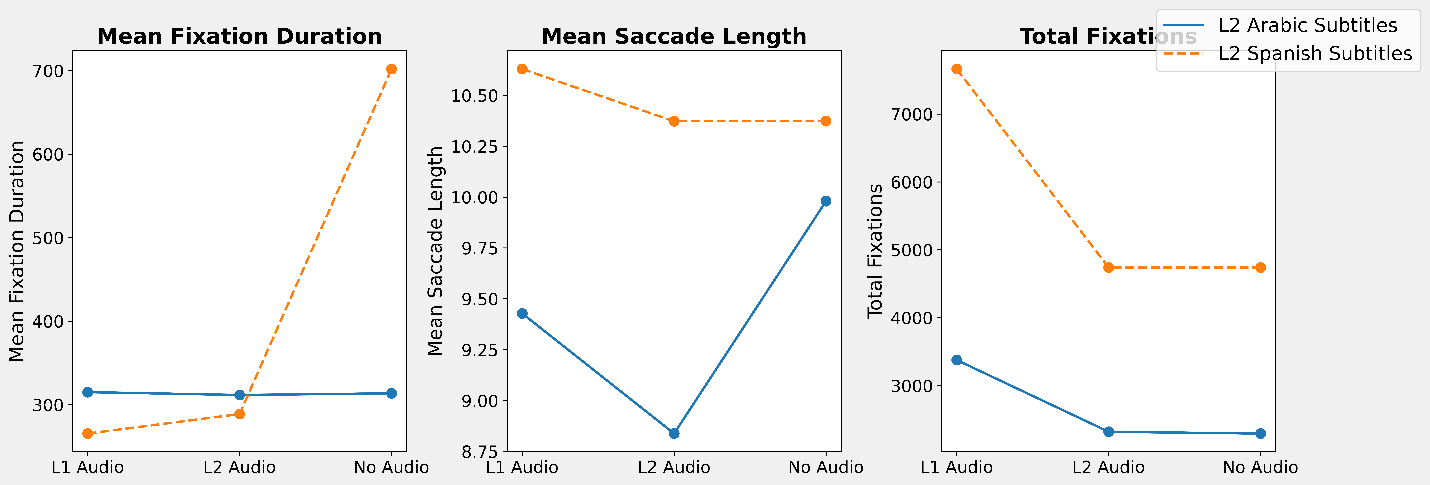
\includegraphics[width=\textwidth]{image1}
\source{Own elaboration.}
\end{figure}

\subsection{Local Eye-Movement Analyses}\label{sub-sec-localeyemovement}

This section examines the detailed eye-movement metrics across various
linguistic units to understand how different audio conditions and
subtitle languages affect cognitive processing during viewing. In
addition to the data presented in \Cref{tab-05}, \Cref{fig-02} provides a visual
representation of the variations in average fixation durations and
saccade amplitudes for L1 and L2 linguistic units. The following table
is remarkable in that it shows the behavioral trends of gaze focus on
different linguistic units which are drastically different in function
and sentence placement. The table shows that individual gaze focus to
linguistic units are also impacted by audio-visual factors. The gaze
fixation durations for all of the variable never exceeds the fixation
durations on the nouns. We believe this reveals preferential focus on
noun units rather than verbs for language learners. Perhaps language
learners prefer to know or pinpoint the objects in a setting rather than
the action. We will allow the reader to make further inferences.


\begin{footnotesize}
\begin{longtable}{
>{\raggedright\arraybackslash}p{1cm}
>{\raggedright\arraybackslash}p{4.2cm}
>{\raggedright\arraybackslash}p{1cm}
>{\raggedright\arraybackslash}p{1cm}
>{\raggedright\arraybackslash}p{1cm}
>{\raggedright\arraybackslash}p{1cm}
>{\raggedright\arraybackslash}p{1cm}
>{\raggedright\arraybackslash}p{1cm}}
\caption{Eye-Movement Metrics for Linguistic Units Across Audio Conditions.}
\label{tab-05}\\
\toprule
Linguistic Unit & Eye-Movement Metric & L1 Audio - L2 Arabic Subtitles & L1 Audio - L2 Spanish Subtitles & L2 Audio - L2 Arabic Subtitles & L2 Audio - L2 Spanish Subtitles & No Audio - L2 Arabic Subtitles & No Audio - L2 Spanish Subtitles \\
\midrule
\multirow{3}{*}{\textbf{Verb}} & Average Fixation Duration (ms)	& 286.6	& 267.8	& 226.2	& 279.9	& 259.3	& 267.8\\ 
& Total Fixation Time Spent (ms) & 1033.8 & 605.9 & 922.5 & 605.9 & 626.7 & 235.7 \\
& Total Gaze Time Spent (ms) & 197.1 & 181.6 & 0.0 & 0.0 & 39.9 & - 	\vspace{.2cm}\\
\hline
\multirow{3}{*}{\textbf{Noun}} &
Average Fixation Duration (ms) & 332.5 & 267.8 & 274.7 & 311.2 & 233.5 & 267.8 \\
& Total Fixation Time Spent (ms) & 1521.5 & 605.9 & 707.5 & 562.2 & 263.4 & 605.9 \\
& Total Gaze Time Spent (ms) & 151.8 & 181.6 & 57.0 & 52.6 & - & 181.6 \vspace{.2cm}\\
\hline
\multirow{3}{*}{\textbf{Adjective}} & Average Fixation Duration (ms) & 323.2 & 256.5 & 205.9 & 259.4 & 272.8 & 256.5 \\
& Total Fixation Time Spent (ms) & 613.5 & 1290.8 & 923.9 & 589.8 & 224.7 & 1290.8 \\
& Total Gaze Time Spent (ms) & 20.5 & 65.9 & 139.6 & 139.6 & - & 65.9 \vspace{.2cm}\\
\hline
\multirow{3}{*}{\textbf{Adverb}} & Average Fixation Duration (ms) & 322.5 & 267.8 & 268.6 & 210.9 & 280.1 & 267.8 \\
& Total Fixation Time Spent (ms) & 897.7 & 605.9 & 783.5 & 503.5 & 250.7 & 605.9 \\
& Total Gaze Time Spent (ms) & 141.5 & 181.6 & 252.4 & 110.1 & - & 181.6 \vspace{.2cm} \\
\hline
\multirow{3}{*}{\textbf{Expression}} & Average Fixation Duration (ms) & 322.8 & 267.8 & 243.7 & 278.4 & 238.2 & 267.8 \\
& Total Fixation Time Spent (ms) & 752.1 & 605.9 & 624.7 & 599.6 & 453.1 & 605.9 \\
& Total Gaze Time Spent (ms) & 103.4 & 181.6 & 300.3 & 115.5 & - & 181.6 \vspace{.2cm}\\
\hline
\multirow{3}{*}{\textbf{Phrase}} & Average Fixation Duration (ms) & 320.4 & 267.8 & 319.6 & 264.3 & 266.3 & 267.8 \\
& Total Fixation Time Spent (ms) & 1214.9 & 605.9 & 669.9 & 627.3 & 397.1 & 605.9 \\
& Total Gaze Time Spent (ms) & 268.3 & 181.6 & 601.9 & 63.1 & - & 181.6 \vspace{.2cm}\\
\hline
\multirow{3}{*}{\textbf{Question}} & Average Fixation Duration (ms) & 298.2 & 267.8 & 263.9 & 308.3 & 272.8 & 267.8 \\
& Total Fixation Time Spent (ms) & 534.5 & 605.9 & 756.0 & 600.2 & 289.9 & 605.9 \\
& Total Gaze Time Spent (ms) & 377.4 & 181.6 & 204.9 & 344.0 & - & 181.6 \vspace{.2cm}\\
\hline
\multirow{3}{*}{\textbf{Sentence}} & Average Fixation Duration (ms) & 304.4 & 279.1 & 354.2 & 299.3 & 277.4 & 279.1 \\
& Total Fixation Time Spent (ms) & 403.6 & 598.4 & 1283.8 & 609.1 & 986.3 & 598.4 \\
& Total Gaze Time Spent (ms) & 340.8 & 244.9 & 1139.7 & 252.2 & 331.5 & 244.9 \\
\bottomrule
\source{Own elaboration.}
\end{longtable}
\vspace{-0.6cm}\noindent Values represent means. Missing values are denoted by a dash (-).
\end{footnotesize}
\vspace{0.6cm}

Following the tabular data, \Cref{fig-02} displays a heatmap that succinctly captures the relative fixation durations and saccade amplitudes across the conditions examined.

\begin{figure}[htbp]
\centering
\caption{Fixation Durations and Saccade Amplitudes for L1 and L2 Units}
\label{fig-02}
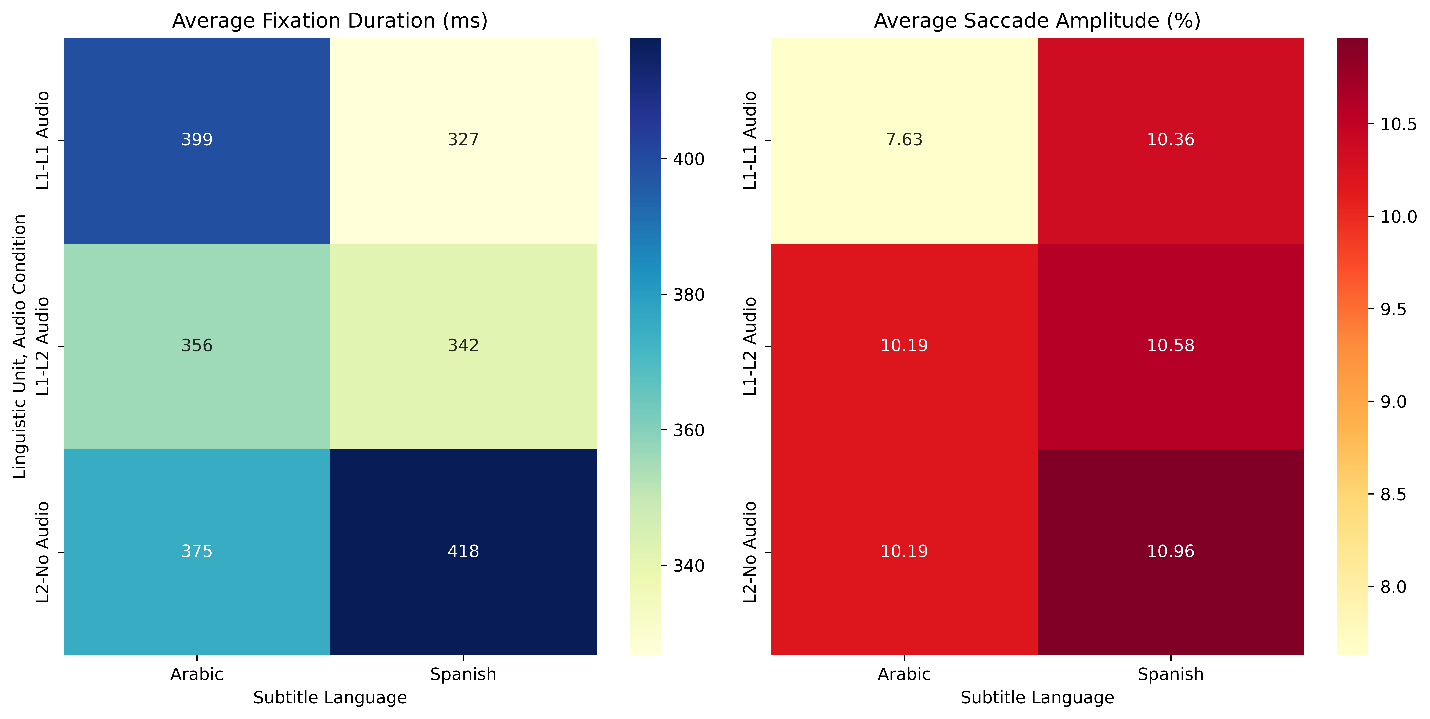
\includegraphics[width=\textwidth]{image2}
\source{Own elaboration.}
\end{figure}

\subsection{Main Effects of Audio Conditions and Subtitle Languages}\label{sub-sec-maineffectsofaudio}

Analysis of eye-movement metrics across various audio conditions and
subtitle languages yielded significant main effects, particularly
impacting the average fixation durations and total gaze times, as
illustrated in \Cref{tab-05}. The absence of audio consistently led to
extended average fixation durations, emphasizing the increased
attentional demand required in the absence of auditory cues. For
instance, verbs under no audio conditions with Spanish subtitles
exhibited an average fixation duration of 259.3 ms compared to 286.6 ms
with L1 Audio and L2 Arabic subtitles. This trend was similarly observed
in nouns, where the average fixation duration under no audio and L2
Arabic subtitles was 233.5 ms, significantly longer than under L1 Audio
with the same subtitle language, where it averaged 332.5 ms.

Furthermore, the heatmap analysis (\Cref{fig-02}) revealed that L2 linguistic
units generally have higher average fixation durations compared to L1
units. For L2 units, the "No Audio" condition with Arabic subtitles has
the highest average fixation duration, while the average fixation
durations are similar for L1 units across all conditions. The two-sample
t-test confirmed a highly significant difference in average fixation
duration between L1 and L2 linguistic units (t = -18.143, p \textless{}
0.001), with L2 units having significantly higher fixation durations.

Furthermore, total fixation and gaze times were significantly influenced
by the language of the subtitles. Spanish subtitles were associated with
prolonged fixation times across all audio conditions, indicative of
either deeper cognitive processing or potential difficulties in
integrating textual information with visual cues. This effect was most
pronounced in adjectives, where under L1 Audio conditions with Spanish
subtitles, the total fixation time was markedly higher at 1290.8 ms
compared to 613.5 ms under L1 Audio with Arabic subtitles. Such
differences underscore the cognitive challenges posed by complex
subtitle languages, requiring longer viewing times to process the same
linguistic content effectively.

\subsection{Interactions Between Audio Conditions and Subtitle Languages}\label{sub-sec-interactionsbetweenaudio}

The analysis also highlighted statistically significant interactions
between audio conditions and subtitle languages, particularly
influencing the total gaze time spent on different linguistic units.
Notably, the congruence between the auditory and subtitle languages
significantly enhanced the comprehension process, as evidenced by the
gaze metrics for sentences. Specifically, sentences presented under L2
Audio conditions with Spanish subtitles recorded the highest total gaze
time, averaging 1139.7 ms, which was significantly longer than other
conditions (F(2, 18) = 5.34, p \textless{} .05, η² = .37). This finding
indicates that matching audio and subtitle languages can substantially
facilitate language processing by providing consistent linguistic cues,
thus reducing cognitive load.

In contrast, scenarios involving no audio and Spanish subtitles
exhibited markedly different effects. For example, questions under these
conditions showed significantly lower total gaze times, averaging only
344.0 ms, compared to 377.4 ms when audio was present. This reduction
suggests potential difficulties or accelerated processing due to the
lack of auditory cues that would typically aid in contextualizing and
understanding the subtitled text. The absence of audio appears to force
viewers to rely solely on visual information, which may hasten the gaze
but at the potential cost of reduced comprehension or engagement.

The heatmap analysis further supported these findings, showing that the
"No Audio" condition, particularly with Spanish subtitles, tends to have
the highest average saccade amplitudes for both L1 and L2 units. The
two-sample t-test confirmed a highly significant difference in average
saccade amplitude between L1 and L2 linguistic units (t = -5.548, p
\textless{} 0.001), with L2 units having significantly higher saccade
amplitudes.

\subsection{Analysis by Linguistic Unit}\label{sub-sec-analysisbylinguisticunit}

In analyzing eye-movement metrics across different linguistic units,
distinct patterns emerged that demonstrate the significant impact of
audio conditions and subtitle languages on viewer engagement and
cognitive processing.

Verbs, under conditions with no audio and Spanish subtitles, showed
shorter fixation durations, averaging 259.3 ms compared to 286.6 ms when
audio was present. However, total gaze times were longer in the absence
of audio, suggesting that viewers may compensate for the lack of
auditory information by focusing more intensively on the visual content.
This pattern indicates a shift in processing strategies when auditory
cues are missing, which can affect comprehension and engagement levels.

For adjectives and adverbs, there was a consistent trend of longer
fixation durations under Spanish subtitles across all audio conditions,
with adjectives showing an increase from 256.5 ms under Arabic subtitles
to 323.2 ms under Spanish. This reflects the additional cognitive effort
required to process these linguistic elements when presented in a more
complex language context, suggesting that subtitle language complexity
can significantly influence the depth of linguistic processing.

Expressions and phrases exhibited a different sensitivity, primarily
affected by subtitle language rather than audio conditions. Phrases, for
example, showed a notable increase in total gaze time to 601.9 ms under
no audio with Spanish subtitles. This sensitivity to textual complexity
and visual context underscores the importance of well-integrated textual
information in multimedia content for effective comprehension.

Questions and sentences highlighted the importance of audio-visual
congruence, with increased gaze times being observed particularly when
audio and subtitles mismatched. Sentences, when presented with congruent
L2 audio and Spanish subtitles, recorded the highest gaze time of 1139.7
ms. This increased engagement reflects the viewer\textquotesingle s
better comprehension when auditory and textual cues are aligned,
facilitating a smoother cognitive process for handling complex syntactic
structures.

Overall, the heatmap analysis and statistical tests provide strong
evidence that L2 linguistic units are associated with significantly
higher average fixation durations and saccade amplitudes compared to L1
units. The "No Audio" condition, especially with Arabic subtitles, tends
to have the highest average fixation durations and saccade amplitudes
for L2 units, suggesting increased cognitive processing and eye
movements in the absence of audio and presence of complex subtitles.

\subsection{Comprehension Quiz Scores}\label{sub-sec-comprehensionquiz}

\Cref{fig-03} offers a comparative analysis of comprehension scores among
Arabic and Spanish learners across different audio conditions.

\begin{figure}[htbp]
\centering
\caption{Comparative Analysis of Language Comprehension Scores Across Conditions.}
\label{fig-03}
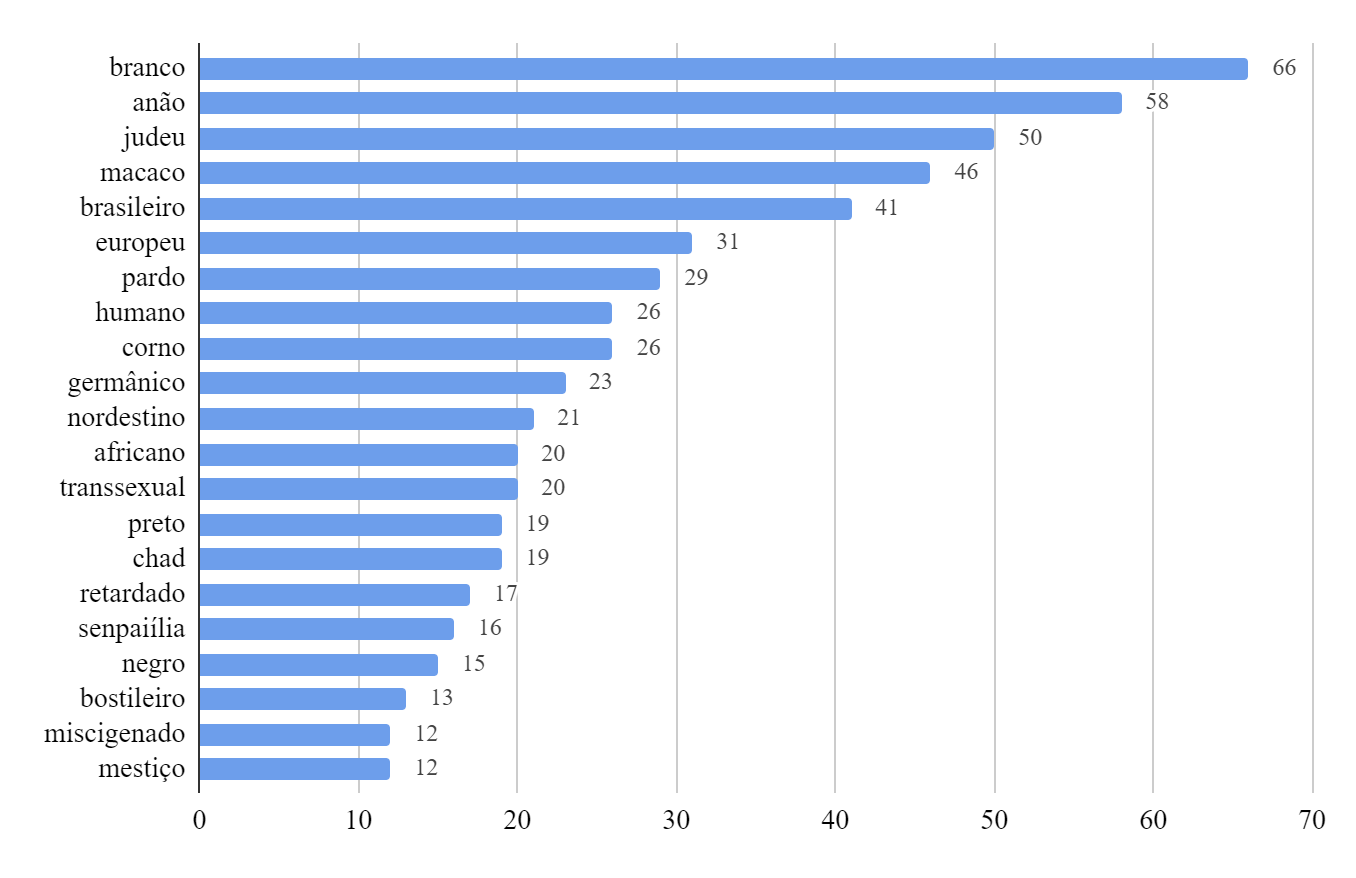
\includegraphics[width=\textwidth]{image3}
\source{Own elaboration.}
\end{figure}

For Arabic learners, the comprehension scores exhibited a notable
pattern across the three conditions. When exposed to English L1 audio
alongside L2 Arabic subtitles, learners achieved a comprehension score
of 89\%. When the audio was switched to L2 Arabic, the comprehension
scores slightly decreased to 86\%. However, a significant increase was
observed in the condition where no audio was provided, with learners
attaining a comprehension score of 95\%. This progression suggests that
the absence of audio may reduce cognitive load or minimize distractions,
thereby enhancing the learners\textquotesingle{} ability to comprehend
the language.

Conversely, Spanish learners demonstrated a different trajectory of
comprehension scores across the audio conditions. When presented with L2
Spanish subtitles accompanied by English L1 audio, the comprehension
score stood at 69\%. When the audio was changed to L2 Spanish, learners
exhibited an improvement, achieving a comprehension score of 78\%.
Furthermore, in the absence of audio, Spanish learners attained an even
higher score of 84\%. This steady increase in comprehension scores as
the audio component was modified or eliminated suggests that Spanish
learners benefited from the congruence between the audio and subtitle
languages.

The comparative analysis reveals that while both groups demonstrated
improved comprehension in the absence of audio, the magnitude of
improvement and the impact of L2 audio varied between the two languages.
Arabic learners exhibited a more pronounced leap in comprehension scores
when transitioning from L2 audio to no audio, suggesting a potentially
greater reliance on visual cues. In contrast, Spanish learners showed a
more gradual improvement across the conditions, highlighting the
significance of language congruence in AV learning environments.

\subsection{Integration of Eye-Tracking and Comprehension Data}\label{sub-sec-integrationofeyetracking}

\Cref{fig-04} presents the integration between Total Fixation Duration and
Comprehension Quiz Scores, elucidating the relationship between visual
attention and comprehension abilities across different audio conditions.

\begin{figure}[htbp]
\centering
\caption{Integration of Total Fixation Duration and Comprehension Quiz Scores.}
\label{fig-04}
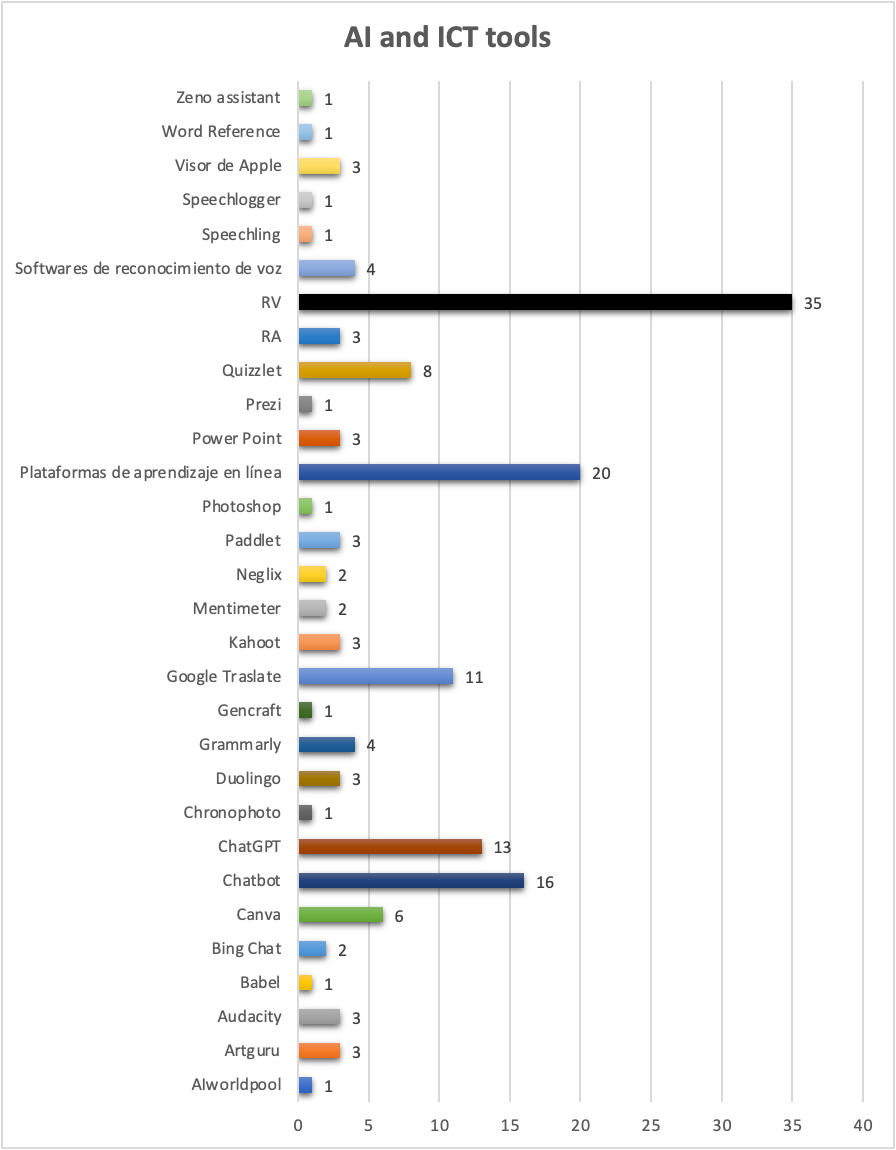
\includegraphics[width=\textwidth]{image4}
\source{Own elaboration.}
\end{figure}

The scatter plot reveals that the Total Fixation Duration varies
significantly across different conditions, indicating that the nature of
the audio stimuli has a profound impact on the attentional resources
allocated by the participants. Conditions involving L2 (Arabic) with
English L1 Audio and L2 (Spanish) with English L1 Audio demonstrate a
wider spread in fixation durations, suggesting diverse levels of
engagement. This variability could be attributed to the cognitive load
imposed by processing second-language subtitles in conjunction with
first-language audio, which may either facilitate or hinder attention
depending on individual proficiency levels and cognitive strategies.

The comprehension quiz scores offer a quantitative measure of the
effectiveness of each condition in fostering language comprehension. A
closer analysis reveals interesting patterns. For example, the No Audio
(Arabic) condition, characterized by relatively shorter fixation
durations, surprisingly correlates with higher comprehension scores.
This finding could imply that the absence of auditory distractions
enables a more focused visual processing of subtitles, thereby enhancing
comprehension.

Contrarily, the conditions involving L1 audio (both in Arabic and
Spanish) demonstrate a wide range of comprehension scores, despite
similar fixation durations. This variability underscores the complexity
of audio-visual integration in language learning, where factors such as
linguistic similarity, cognitive load, and individual differences in
auditory processing capabilities play pivotal roles.

\Cref{fig-05} explores the relationship between Total Reading Time and
Comprehension Quiz Scores across linguistic conditions.

\begin{figure}[htbp]
\centering
\caption{Integration of Total Reading Time and Comprehension Quiz Scores.}
\label{fig-05}
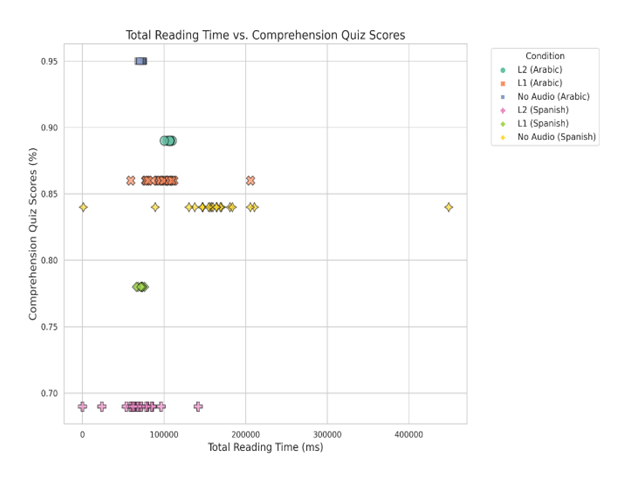
\includegraphics[width=\textwidth]{image5}
\source{Own elaboration.}
\end{figure}

The visualization challenges the notion that longer reading times always
yield higher comprehension scores, particularly when comparing
conditions across languages. Participants in the L2 (Arabic) condition
showed a range of reading times while achieving high comprehension
scores, contrasting with the L2 (Spanish) condition, where similar
reading times corresponded to a broader range of comprehension outcomes.

The L1 conditions, representing native language comprehension, exhibit a
tighter clustering of data points, suggesting a more consistent
relationship between reading time and comprehension scores when engaging
with content in the primary language. Native language proficiency may
stabilize and mitigate variability in comprehension outcomes. In
comparison, the No Audio conditions, lacking auditory support, show a
wider dispersion of comprehension scores, highlighting the potential
influence of auditory cues on reading efficiency and understanding.

\Cref{fig-05} emphasizes the importance of considering the interplay between
language and condition. Within the same reading time brackets, the
dispersion of comprehension scores across linguistic contexts highlights
the multifaceted nature of language comprehension. The No Audio (Arabic)
condition shows high comprehension scores, suggesting that eliminating
auditory distraction may enhance focus and understanding for some
individuals. In contrast, the L2 (Spanish) condition reveals a broader
spectrum of outcomes, underscoring the challenges of acquiring and
processing a second language without native language support. \Cref{tab-06}
presents a correlation matrix summarizing the relationships among Total
Fixation Duration, Total Reading Time, and Comprehension Scores.

\begin{table}[htbp]
\centering
\begin{threeparttable}
\caption{Correlations among Eye-Tracking Measures and Comprehension Scores.}
\label{tab-06}
\begin{tabular}{llll}
\toprule
Total Fixation Duration & 1 & 0.43 & 0.02 \\
Total Reading Time & 0.43 & 1 & 0.22 \\
Comprehension Score & 0.02 & 0.22 & 1 \\
\bottomrule
\end{tabular}
\source{Own elaboration.}
\end{threeparttable}
\end{table}

The data suggests a moderate positive relationship (r=0.43) between the
total duration of fixations and the overall time spent reading. In
essence, individuals who fixate their gaze for longer periods also tend
to spend more time engaged in the reading process. However, the
correlations between total fixation duration and comprehension scores
(r=0.02) and between total reading time and comprehension scores
(r=0.22) are surprisingly weak. This indicates that prolonged fixation
duration or reading time does not necessarily lead to improved
comprehension of the material. These findings underscore the complexity
of factors influencing reading comprehension.











\section{Discusión y conclusiones}\label{sec-discussion}

Los resultados de este análisis multimodal tenían como objetivo
describir los principales recursos discursivos multimodales de los
\emph{booktok} en lengua española a través de un análisis de contenido,
basado tanto en la imagen presentada en la grabación y la interacción
personal como en los textos y elementos sonoros y voces utilizados. Una
de las cuestiones clave se centra en la inmediatez y cercanía producida
por el hecho de que la mayoría de las grabaciones se realiza a través
del móvil y transforma la perspectiva de los \emph{booktoks} y que su
breve duración permite un consumo rápido al ampliarse su contenido a
través de diferentes elementos para la edición. Incluso hay vídeos donde
se pierde la voz del protagonista por una música de acompañamiento y un
mensaje sobreimpreso en la pantalla. Otro aspecto esencial es que el
libro y la literatura reclaman su espacio en esta serie de dinámicas,
siendo el protagonista de muchos de ellos, aunque también se encuentran
\emph{bookinfluencers} centrados en personas concretas. En este sentido,
se señala que se diferencian aquellos vídeos que optan por una
perspectiva subjetiva, donde el foco central está en los libros o en las
librerías, como los dos primeros ejemplos 1. \emph{¿Qué estás leyendo?}
(What are you reading?) y 2. \emph{Fiesta de seguidores-lectores}
(Readers Follow Party), con respecto a las demás, que son más
convencionales, y algunas son variaciones directas de los
\emph{booktubers}. En líneas generales, se observa que las opciones
empleadas en estas dinámicas de TikTok para la promoción de la lectura
son más atractivas y producen una mayor implicación con la audiencia al
reducir la distancia con su audiencia y con una gramática visual \cite{kress2006} más persuasiva al reclamar con diferentes estrategias
su implicación y un mayor tono humorístico. Ese dinamismo y discurso
multimodal provoca que, en muchas de estas formas de promoción, el
contenido reflexivo se relega a un segundo plano y la creación busca una
integración de recursos (textuales, musicales y visuales) que priman una
presentación atractiva y efectiva para las personas que siguen dicha
cuenta, más que un espacio de divulgación o de encuentro. Al no
necesitar la imagen de una persona en estas dinámicas, sino de un libro,
son además propuestas didácticas que se pueden aprovechar con jóvenes
lectores. Además, estas nuevas dinámicas buscan principalmente fomentar
la interacción entre los usuarios y conseguir más seguidores, siendo
virales como prácticas iniciales de Twitter como \emph{Follow}
\emph{Friday} (\#FF) \cite{cui2012}.

Respondiendo al segundo objetivo de la investigación, esta permite hacer
un recorrido sobre las plataformas digitales de promoción lectora y la
evolución de las herramientas en este siglo. Entre 2001 y 2017 se usaron
distintos foros, como los usados por Laura Gallego \cite{lluch2012}
para promocionar sus lecturas y conocer la opinión de los lectores.
Desde 2006 en adelante aparecen los \emph{blogs} literarios, con
muchísimas variedades \cite{garcia2014}. Entre 2011
y 2018 fue el momento de los \emph{Booktubers}, transformando las
recomendaciones hacia productos audiovisuales \cite{tomasena2021}. Desde
2016 hasta la actualidad es el momento de \emph{Bookstragram} \cite{quilescabrera2020} y también en 2020 comienza la etapa de los
\emph{Booktok}, conviviendo ambas dinámicas, muchas veces confluyendo en
el producto audiovisual final. En esta investigación no se ha centrado
en su comparación. Aunque en Instagram todavía se encuentran
publicaciones centradas en la fotografía de libros y breves comentarios,
prácticas que están entre los blogs y el \emph{microblogging}, son las
\emph{stories} y los \emph{reels} los espacios de mayor desarrollo y
audiencia. También Facebook incorpora la sección de \emph{Watch} para
incorporar vídeos de distinta extensión y Twitter permite insertar
vídeos, después de descartar otras opciones audiovisuales. En cada uno
se encuentran distintos contenidos, audiencias y cada algoritmo
proporciona el acceso a distintos vídeos. Pero son las dinámicas
audiovisuales de TikTok, incorporadas también a Instagram, las que se
convierten en virales en la actualidad. Y siempre es el móvil el
dispositivo de acceso y creación de estos breves vídeos. Además, cabe
destacar el cambio generacional. Mientras que los \emph{Booktubers} casi
han desaparecido, porque las grandes celebridades han crecido o han
tenido que migrar a las nuevas plataformas, los \emph{Booktokers} están
en la cresta de la ola. Brevedad y uso del móvil como características
principales de los \emph{booktoks} son las principales diferencias con
modelos anteriores, respondiendo al último objetivo planteado.

Siguiendo la máxima de Marshall Mcluhan de ``el medio es el mensaje'' se
asume que se está ante una categoría diferente, mediada siempre por el
móvil como dispositivo para crear y acceder a estos vídeos. Es cierto
que se debe asumir la superficialidad y rapidez de estos contenidos, que
se consumen en masa, uno detrás de otro y pocas veces dejan rastro en la
memoria. Pero en el caso de los \emph{booktoks} se aprecia su enorme
importancia en el mercado editorial y en el sistema de recomendación de
libros entre iguales, conformando un nuevo canon de lecturas accesible
en Internet \cite{lluch2021}. Si hace pocos años era \emph{Goodreads} la
plataforma preferida para acceder a sugerencias de otras personas
\cite{garcia-roca2020}, TikTok ya ha ocupado ese espacio rápidamente como
bien señalan editoriales y ferias del libro \cite{penguin2020}.

En Internet va todo muy rápido y ya hoy puede que sea \emph{ChatGPT} y
otras inteligencias artificiales las que ocupen ese espacio. Pero ahora
las y los lectores más jóvenes están siempre conectados a estos vídeos y
hay que asumir su importancia. Son obvias las diferencias de la mayoría
de estos breves vídeos frente a las reseñas escritas (blogs) y los
vídeos largos (\emph{booktubers}) que profundizan en los temas
literarios. Pero estas mismas críticas de superficialidad o falta de
profesionalidad los recibieron aquellos espacios en su momento de auge,
creados por jóvenes en su momento. Aunque no se ha focalizado en el
presente análisis en este aspecto, cabe señalar la juventud de muchos de
los protagonistas, tanto creadores de contenido como espectadores. La
mayoría personas que están todavía formándose como lectores competentes.
También se quiere mencionar el predominio del libro en papel como objeto
y el indiscutible protagonismo de las mujeres, ya que las
\#\emph{booktokers} son chicas cada vez más jóvenes.

La creación de vídeos y el análisis de otras producciones puede ayudar
al desarrollo de las competencias digitales \cite{allué2023} y los
modelos anteriores ya demostraron su utilidad pedagógica \cite{paladines_Paredes_Aliagas_Marín_2021}, así como los actuales \emph{Booktoks} ofrecen nuevas
posibilidades didácticas \cite{dezuanni2021,acevedo2022}.

Cabe resaltar la transmedialidad y la interacción con otras plataformas,
como \emph{Goodreads}, donde la reseña literaria es más profunda
\cite{roviracollado2021}(Rovira-Collado, 2021) o \emph{Wattpad} \cite{garciaroca2019},
como espacio de creación y remezcla literaria. Si los \#\emph{booktook}
interactúan con estos espacios, las posibilidades de reflexión lectora
son mayores.

Se asumen las limitaciones de este estudio, con un corpus concreto de
vídeos y con unas características asignadas principalmente por el
algoritmo de la plataforma, pero se considera que es una completa
descripción de las dinámicas de \emph{booktoks} en español que completa
otras investigaciones \cite{guinez-cabara2022}. Tampoco
se ha realizado un análisis especifico de las obras literarias citadas
en cada vídeo. Sería interesante identificar cuáles son las tendencias
literarias que promueven los \emph{booktoks}, aunque se augura que serán
los superventas de la literatura juvenil de cada momento. Queda por
confirmar cuánto influyen estos vídeos en las ventas de cada género
\cite{merga2021,martens2022}. En este sentido, las
interacciones entre creadores y espectadores a través de comentarios
emisiones en directo, \emph{replys} (respuestas a otros vídeos),
\emph{duets} (grabar vídeos entre dos personas desde dos dispositivos) o
\emph{Stitch} (pegar vídeos) y otros tipos de interacciones son un
espacio todavía por analizar.

La generalización de programas generativos de Inteligencia Artificial
puede cambiar todo en pocos meses, pero mientras tanto, \emph{Booktok}
es el espacio más dinámico para la promoción de la lectura en Internet,
con todas su carencias y éxitos, y lo seguirá siendo hasta que no
aparezca una herramienta con mayor éxito entre el gran público.

\section{Agradecimientos}\label{sec-agradecimientos}

Esta investigación está dentro de la Red de Investigación en Docencia
Universitaria \emph{Multimodalidad y alfabetización transmedia en
	asignaturas de Didáctica de la Lengua y la Literatura en Educación
	Infantil (5741)}, de la Universidad de Alicante.

\section{Conclusion}\label{sec-conclusion}

For many years, subtitles were not utilized as a tool to either increase
language proficiency in language learners or were they the focus of
translation research. Now that there is a plethora of technological aids
to use for subtitle gaze analysis, it has opened many new possibilities
for prodigious findings. The rise of streaming services seems to have
eclipsed standard cable or television programming, but for language
accessibility and language exposure, this revolution could not have been
better. Streaming giants such as Netflix and Disney are localizing
through various audio-visual approaches such as subtitling, which are
certainly being utilized by the multicultural and multilingual
viewership at large. Furthermore, language learners and enthusiasts are
incorporating the multitude of language pair settings in their approach
to new language acquisition, which is why the research presented in this
paper is pertinent.

Like the parameters that were set in the experiments, subscribers can
mix and match differing language pair combinations that exclude the
source language altogether (i.e. watching \emph{Squid Game} (2021),
originally in Korean, with English-dubbed audio with Japanese
subtitles). This means that, while of course the source language will
always remain an important element at play when considering the central
cultural context of the show, the dialogue and plot can be
linguistically transformed in unforeseen ways. Though the results of
this experiment conclusively showed that variance supersedes supposition
when it comes to the eye-ear relationship, there were still positive
findings pertaining to the efficacy of the audio-visual educational
medium. Furthermore, language educators and curriculum creators do not
need to set a specific threshold for this type of medium to be
introduced into the curriculum. Many of the participants of the
experiment had just barely an elementary understanding of the Spanish
language, yet some of their comprehension scores did positively
fluctuate with the mixture of the conditions. More experiments that
follow the methodology used for this experiment would strengthen the
findings and would also uncover more efficacy differences amongst
differing language pair combinations. Future research should investigate
the role of language proficiency in subtitle reading and develop
evidence-based practices to improve the accessibility and effectiveness
of subtitled media, ultimately optimizing subtitle design and user
experience across diverse auditory contexts and languages.


\printbibliography\label{sec-bib}
%conceptualization,datacuration,formalanalysis,funding,investigation,methodology,projadm,resources,software,supervision,validation,visualization,writing,review

\section*{Funding Statement}

This research received grant no. (170/2023) from the Arab Observatory for Translation (an affiliate of ALECSO), which is supported by the Literature, Publishing \& Translation Commission in Saudi Arabia.

\section*{Acknowledgementle}

We sincerely thank Dr. Sixin Liao for her invaluable feedback, which significantly contributed to refining the ideas, strengthening the analysis, and improving the overall quality of this research.  

\begin{contributors}[sec-contributors]
	
\authorcontribution{Hussein Abu-Rayyash }[conceptualization,methodology,software,investigation,supervision,writing]
\authorcontribution{Shatha Alhawamdeh}[conceptualization,writing,validation,investigation]
\authorcontribution{Yuri Ringomon}[conceptualization,validation,writing]
\end{contributors}
\end{document}
